\section{Einleitung}
\subsection{Einführung in die Thematik}
\blindtext\nomenclature{W3C}{World Wide Web Consortium}
\blindtext\footcite[Vgl.][]{mswpf}\footcite[Vgl.][19]{sadtler_rechtskonformes_2017}

\subsection{Problemstellung und Zielsetzung}
\blindtext

\subsection{Methodischer Aufbau der Arbeit}
\blindtext

\section{Hauptteil}
\subsection{LaTeX-Beispiele und Befehle}
„Dies ist ein direktes Zitat."\footcite[][224]{mertens_digitalisierung_2017} \blindtext\footcite[Vgl.][]{msdatabind}\footcite[Vgl.][]{lambda}\footcite[Vgl.][34]{Digitaloekonomie}
\blindenumerate
\blindtext\footcite[Vgl.][415-426]{Tanenbaum2016}\footcite[Vgl.][223]{mandl_internet_2019}

\begin{figure}[!htb]
    \caption{Terminal}
    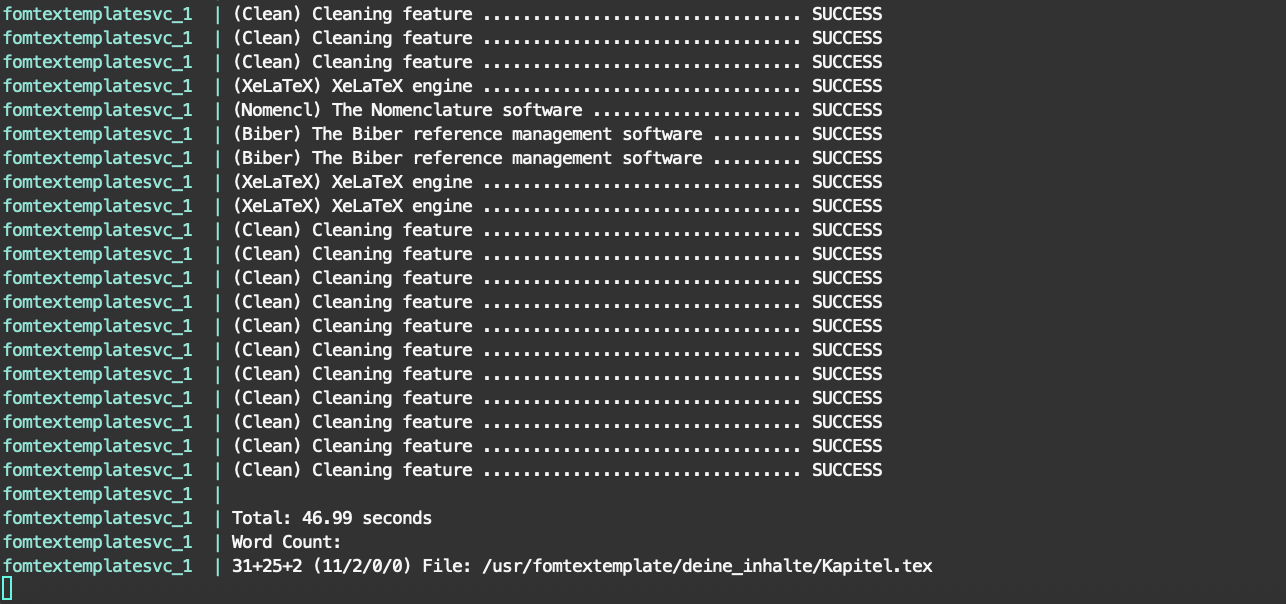
\includegraphics[width=1\textwidth]{.github/terminal}
    \captionsetup{width=1\textwidth}
    \capquelle{\cite[][200]{bsp}}\label{abb_bsp}
\end{figure}
\blindtext

\subsubsection{Tabelle}
\Blindtext\footcite[Vgl.][34]{Digitaloekonomie}\footcite[Vgl.][]{mesh}
\blinditemize
\blindtext (vgl. Tabelle \ref{tabelle_eins}).\footcite[Vgl.][511]{Tanenbaum2016}
\begin{table}[!htb]\label{tabelle_eins}
    \setlength{\arrayrulewidth}{1pt}
    \begin{threeparttable}
        \caption{Tabelle Eins}
        \begin{tabularx}{\textwidth}{|X|X|X|X|X|}
            \hline
            Spalte 1 & Spalte 2 & Spalte 3 & Spalte 4 & Spalte 5 \tabularnewline \hline
            1 & 2 & 3 & 4 & Lorem ipsum dolor sit amet \tabularnewline \hline
            1 & 2 & 3 & 4 & Lorem ipsum dolor sit amet \tabularnewline \hline
            1 & 2 & 3 & 4 & Lorem ipsum dolor sit amet \tabularnewline \hline
        \end{tabularx}
        \begin{tablenotes}[flushleft]
            \item \normalsize{Quelle: \cite[][207]{bsp}}
        \end{tablenotes}
    \end{threeparttable}
\end{table}

\subsubsection{Quelltext}
\lstinputlisting[caption={Writing Templates}\label{Templates},language=Yaml]{deine_inhalte/Quellcode/red_hat.yaml}
\captionsetup{width=1\textwidth}
\capquelle{\cite[][]{red}}\label{Red Hat} \\


\subsubsection{LaTeX-Befehle}
    \textnormal{Normale Schrift} 
    \textbullet\addspace \textbf{fette Schrift} 
    \textbullet\addspace \textit{kursive Schrift} 
    \textbullet\addspace \textsl{schiefe Schrift} 
    \textbullet\addspace \underline{unterstrichen} 
    \textbullet\addspace \texttt{Schreib\-ma\-schi\-ne} 
    \textbullet\addspace \textsf{Sans Serif} 
    \textbullet\addspace \textrm{Roman} 

\subsection{Test: Silbentrennung - Gegenüberstellung - darf nicht in den weißen Rand laufen}
Im zweiten Kapitel wird zunächst der Begriff \textit{Bring Your Own Device} (BYOD) definiert. Darauffolgend wird dargelegt welche Fokusse gesetzt werden sollen und Schlussfolgerungen gezogen, sowie eine Sicherheitsrichtlinie abgeleitet. Welche als Grundlage einer Gegenüberstellung mit etablierten Konzepten dient, sodass Strategien erörtert werden können. 

\section{Test der Ebenen und Beispieldiagramme}
\subsection{Ebene 2}
\blindtext
\begin{figure}[!htb]
  \caption{Continuous Integration Prozess}
  \captionsetup{width=1\textwidth}
  \smartdiagramset{
    border color=teal,
    uniform color list=teal!60 for 6 items,
    uniform arrow color=true,
    arrow color=gray!80,
    back arrow disabled=true
  }
  \smartdiagram[flow diagram:horizontal]{Develop \& Commit,Build,Integration,Build on Integrated Code, Integration-Tests,Packing}
  \capquelle{Eigendarstellung angelehnt an \cite[][19-20]{pathania_learning_2017}}\label{Continuous Integration Prozess}
\end{figure}
\subsection{Ebene 2.2}
\blindtext

\begin{figure}[!htb]
  \caption{Testpyramide}
  \captionsetup{width=1\textwidth}
  \begin{center}
    \begin{tikzpicture}
      \node [double arrow, draw, draw=teal, fill=teal!20, very thick, rotate=90] 
          at (-5.5,2.3) {Isolation | Integration};
      \node [double arrow, draw, draw=teal, fill=teal!20, very thick, rotate=90] 
          at (5.5,2.3) {Schnell\:\:\:\:|\:\:\:\:Langsam};
      
      \coordinate (A) at (-5,0) {};
      \coordinate (B) at (5,0) {};
      \coordinate (C) at (0,4.5) {};
      \draw[name path=AC, draw=teal, very thick] (A) -- (C);
      \draw[name path=BC, draw=teal, very thick] (B) -- (C);
      \foreach \y/\A in 
          {
            0/Unit Tests,
            1.25/Service Tests,
            2.5/UI Tests
          }
          { %0/G,1/F,2/E,3/D,4/C,5/B,6/A
            \path[name path=horiz] (A|-0,\y) -- (B|-0,\y);
            \draw[draw=teal, very thick, 
              name intersections={of=AC and horiz,by=P},
              name intersections={of=BC and horiz,by=Q}
            ] (P) -- (Q)
            node[midway,above] {\A};
          }
    \end{tikzpicture}
  \end{center}
  \capquelle{Eigendarstellung angelehnt an \cite[][311-317]{cohn_succeeding_2010}}\label{Testpyramide}
\end{figure}

\subsubsection{Ebene 3}
\blindtext
\subsubsection{Ebene 3.2}
\blindtext
\subsubsubsection{Ebene 4}
\blindtext
\subsubsubsection{Ebene 4.2}
\blindtext
\footcite[Vgl.][79]{Schelinski2019}

\section{Schluss}
\subsection{Fazit}
\blindtext (vgl. Abbildung \ref{abb_bsp}).

\subsection{Ausblick}
\blindtext
